% Generated by experiments/export_latex.py -- do not edit by hand.
% Regenerate with: make paper-tables

\definecolor{nace}{HTML}{2A78D6}
\definecolor{news}{HTML}{EB6834}
\definecolor{gridline}{HTML}{E1E0D9}
\definecolor{axisline}{HTML}{C3C2B7}
\definecolor{ink2}{HTML}{52514E}
\begin{figure}[t]
\centering
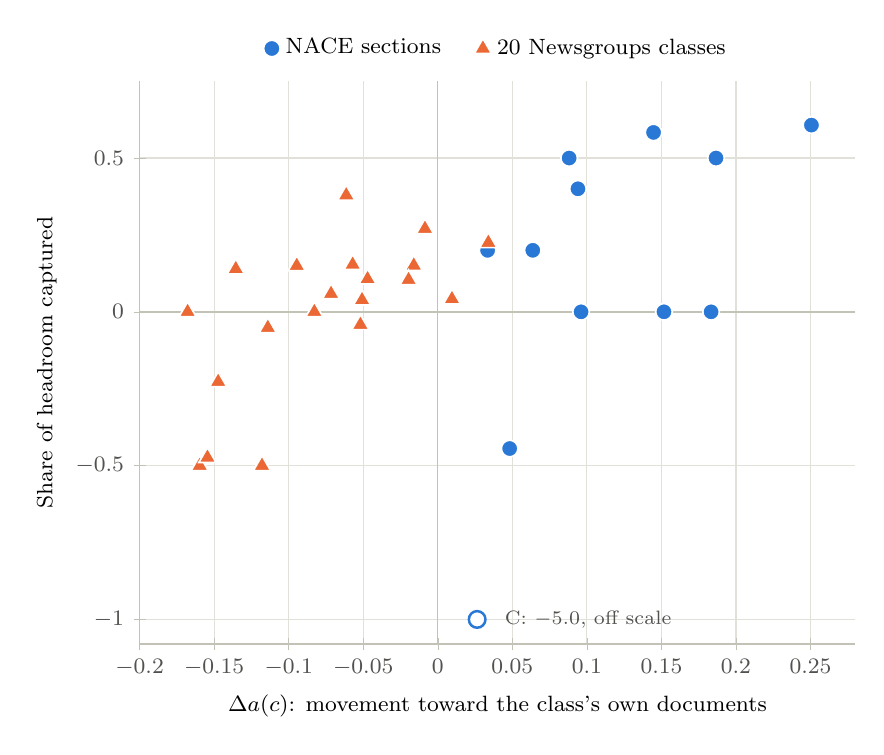
\begin{tikzpicture}
\begin{axis}[
  width=0.88\columnwidth, height=0.72\columnwidth,
  xmin=-0.2, xmax=0.28, ymin=-1.08, ymax=0.75,
  xlabel={$\Delta a(c)$: movement toward the class's own documents},
  ylabel={Share of headroom captured},
  axis lines=left, axis line style={axisline, -},
  grid=major, major grid style={gridline, line width=0.4pt},
  tick style={axisline}, tick label style={font=\footnotesize, text=ink2},
  label style={font=\footnotesize},
  xticklabel style={/pgf/number format/.cd, fixed, precision=2},
  legend style={font=\footnotesize, draw=none, fill=none, at={(0.5,1.02)}, anchor=south},
  legend columns=2, legend style={/tikz/every even column/.append style={column sep=10pt}},
  legend cell align=left, clip=false,
]
\draw[axisline, line width=0.5pt] (axis cs:0,-1.08) -- (axis cs:0,0.75);
\draw[axisline, line width=0.5pt] (axis cs:-0.2,0) -- (axis cs:0.28,0);
\addplot[only marks, mark=*, mark size=3pt, mark options={fill=nace, draw=white, line width=0.6pt}] coordinates {
  (0.2506,0.6071) (0.0940,0.4000) (0.1517,0.0000) (0.0637,0.2000) (0.0881,0.5000) (0.0482,-0.4444) (0.0961,0.0000) (0.1866,0.5000) (0.1833,0.0000) (0.0334,0.2000) (0.1447,0.5833)
};
\addlegendentry{NACE sections}
\addplot[only marks, mark=triangle*, mark size=3.6pt, mark options={fill=news, draw=white, line width=0.6pt}] coordinates {
  (-0.0716,0.0588) (-0.0519,-0.0417) (0.0095,0.0417) (-0.0161,0.1509) (-0.0196,0.1042) (0.0339,0.2250) (-0.0828,0.0000) (-0.1597,-0.5000) (-0.0571,0.1538) (-0.1678,0.0000) (-0.0614,0.3793) (-0.0086,0.2703) (-0.1545,-0.4737) (-0.0508,0.0385) (-0.1473,-0.2273) (-0.1179,-0.5000) (-0.1355,0.1395) (-0.0946,0.1500) (-0.1140,-0.0517) (-0.0471,0.1067)
};
\addlegendentry{20 Newsgroups classes}
\addplot[only marks, forget plot, mark=*, mark size=3pt, mark options={fill=white, draw=nace, line width=0.9pt}] coordinates {(0.0264,-1.0)};
\node[font=\scriptsize, text=ink2, anchor=west] at (axis cs:0.0384,-1.0) {C: $-5.0$, off scale};
\end{axis}
\end{tikzpicture}
\caption{Each point is one class. Horizontal: how far elaborating its description moved the class vector toward its own documents. Vertical: the share of the available headroom in recall the class captured, $(r_{\mathrm{rich}} - r_{\mathrm{terse}})/(1 - r_{\mathrm{terse}})$. Spearman $\rho = \AlignRho$ over \NCLASSES\ classes ($p = \AlignP$), and the ordering holds within each corpus. A class that falls below the plotted range is drawn on the lower edge with its value.}
\label{fig:alignment}
\end{figure}
